\mansection{set\_diag}
\begin{mandesc}
  \short{set_diag}{set a diagonal of a matrix}
\end{mandesc}
%-- Calling sequence section
\begin{calling_sequence}
\begin{verbatim}
  A.set_diag[v]
  A.set_diag[v,k]
\end{verbatim}
\end{calling_sequence}
%-- Parameters
\begin{parameters}
  \begin{varlist}
    \vname{A}: any kind of matrix
    \vname{v}: vector or scalar (of same type than A)
    \vname{k}: optional argument, the diagonal number (default is $0$)
  \end{varlist}
\end{parameters}

\begin{mandescription}

  This function sets the given diagonal $k$ (0 by default) of a matrix 
with either a vector (which must have as many elements as the given 
diagonal) or with a scalar (the given diagonal is filled with the
scalar).

Remarks:  
\begin{itemize}
\item The matrix element $A_{i,j}$ is located on the diagonal number $j-i$. So main 
diagonal is numbered $0$, the diagonal number $1$ and $-1$ are respectively located just 
upper and under the main diagonal, etc...
  $$
  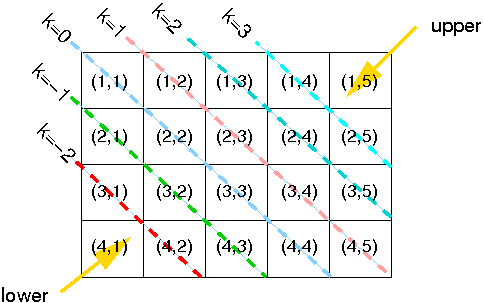
\includegraphics[width=8cm]{\mansrc basicnumarrays/diagonal} 
  $$

\item For a sparse matrix, argument $v$ can be given also using a full vector (or scalar).

\end{itemize}

\end{mandescription}

%--example 
\begin{examples}
\begin{mintednsp}{nsp}
A = zeros(5,5)
A.set_diag[2]; A.set_diag[-1,1];  A.set_diag[-1,-1]; 
print(A)

// same example with a sparse matrix
A = sp_create(5,5)
A.set_diag[2]; A.set_diag[-1,1];  A.set_diag[-1,-1]; 
print(A)

// an example with a IMat
A = imat_create(4,6)
for k=-3:5; A.set_diag[m2i(k),k]; end
print(A)

// an example with a string matrix
A = smat_create(3,3)
A.set_diag["a",-2]
A.set_diag[["b","c"],-1]; 
A.set_diag[["d","e","f"],0]; 
A.set_diag[["g","h"],1]; 
A.set_diag[["i"],2]; 
print(A)
\end{mintednsp}
\end{examples}

%-- see also
\begin{manseealso}
  \manlink{diag}{diag}, \manlink{tril}{tril}, \manlink{triu}{triu}
\end{manseealso}

